\RequirePackage{luatex85}
\documentclass{standalone}
\usepackage{tikz}

% Color Definitions
\definecolor{SourceColor}{RGB}{85,168,104}
\definecolor{TargetColor}{RGB}{221,132,82}
\definecolor{TargetChangerColor}{RGB}{255,153,0}
\definecolor{AbsorbingAreaColor}{RGB}{196,78,82}
\definecolor{ObstacleColor}{RGB}{179,179,179}
\definecolor{StairColor}{RGB}{129,114,178}
\definecolor{MeasurementAreaColor}{RGB}{255,0,0}
\definecolor{InformationAreaColor}{RGB}{0,100,20}
\definecolor{AerosolCloudColor}{RGB}{202,156,76}
\definecolor{AgentColor}{RGB}{76,114,202}
\definecolor{AgentIdColor}{RGB}{255,127,0}

\newcommand{\MeasurementAreaOpacity}{0.549020}
\newcommand{\AerosolCloudOpacity}{0.039216}

\begin{document}



\begin{tikzpicture}
\node[] at (0,0) {
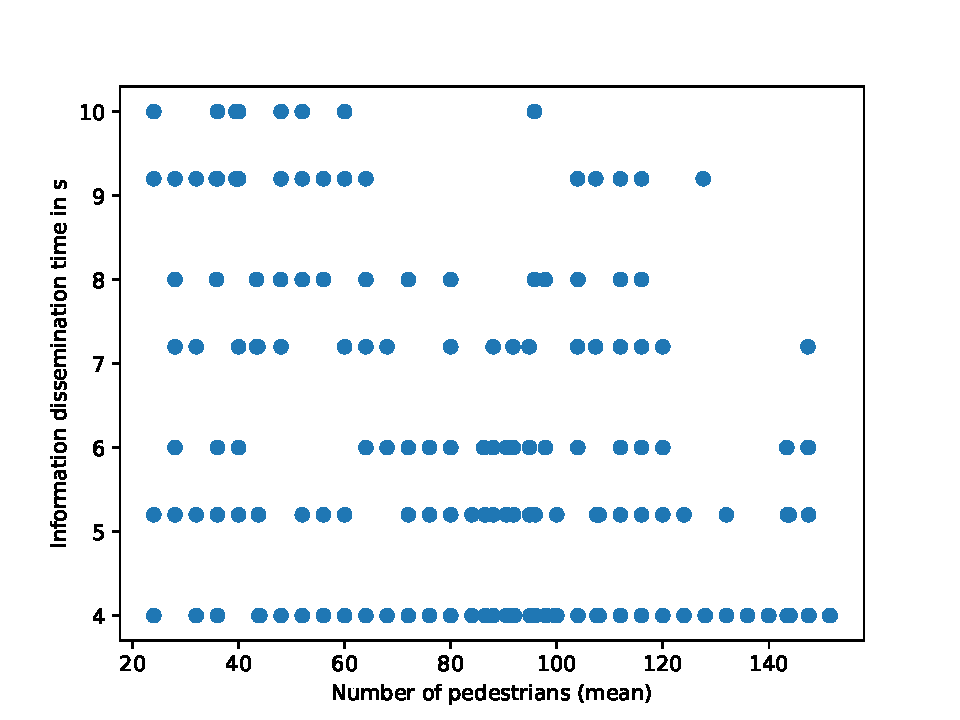
\includegraphics[width=7.5cm]{./Shadowing_results/InfoDisserminationTime.pdf} };
\node[] at (7.5,0) {
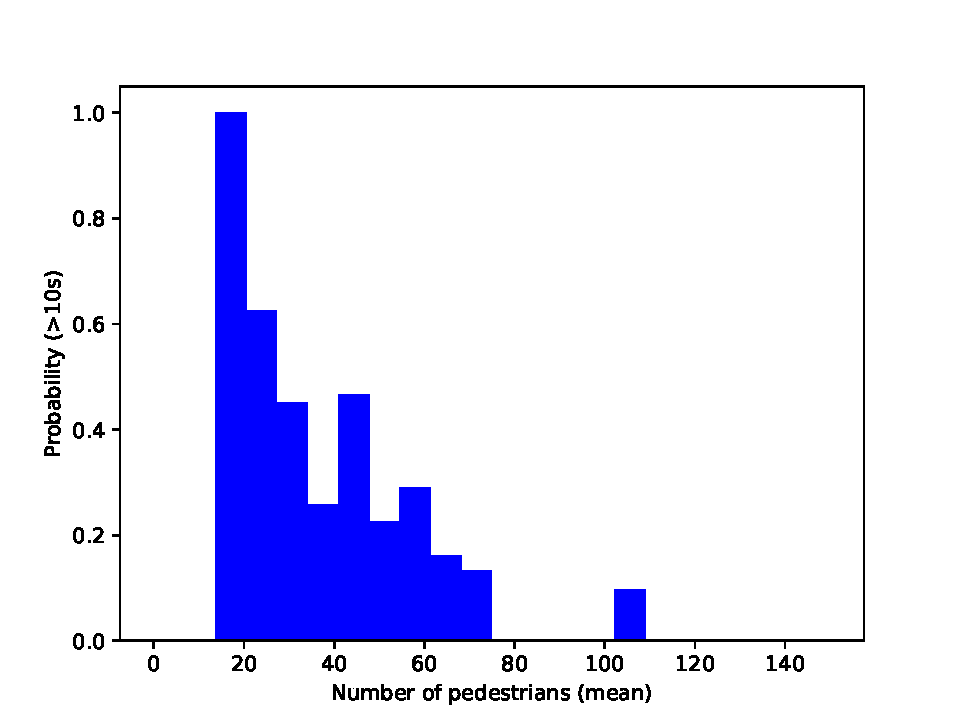
\includegraphics[width=7.5cm]{./Shadowing_results/Probabilites_normed.pdf} };

\node[font=\small, fill=white, text width=4.5cm,rotate=90] at (3.8,0)  {Probability for shadowing ($t_{dissemination} > 10s$)};
\node[font=\small, fill=white, text width=4.5cm,rotate=90] at (-3.6,0)  {  Dissemination time in s \\ ($t_{dissemination} \leq  10s $ only) };
\node[font=\small, fill=white, text width=4.5cm] at (1.2,-2.7)  {  Number of agents };
\node[font=\small, fill=white, text width=4.5cm] at (8.5,-2.7)  {  Number of agents };
\end{tikzpicture}

\end{document}
